

\tikzset{every picture/.style={line width=0.75pt}} %set default line width to 0.75pt        

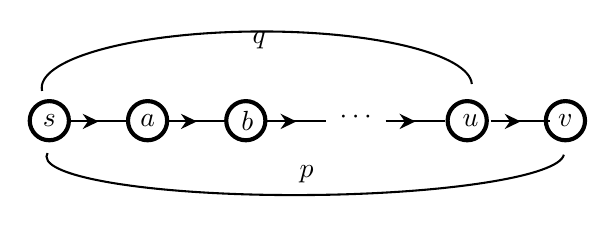
\begin{tikzpicture}[x=0.5pt,y=0.5pt,yscale=-1,xscale=1]
%uncomment if require: \path (0,145); %set diagram left start at 0, and has height of 145

%Straight Lines [id:da30971022934824355] 
\draw [color={rgb, 255:red, 0; green, 0; blue, 0 }  ,draw opacity=1 ][line width=0.75]    (65.5,74) -- (108.5,74) ;
\draw [shift={(87,74)}, rotate = 180] [fill={rgb, 255:red, 0; green, 0; blue, 0 }  ,fill opacity=1 ][line width=0.08]  [draw opacity=0] (11.61,-5.58) -- (0,0) -- (11.61,5.58) -- (7.71,0) -- cycle    ;
%Shape: Arc [id:dp4711929405237] 
\draw  [draw opacity=0] (423.21,98.05) .. controls (419.98,113.6) and (337.66,126.55) .. (236.51,127.21) .. controls (133.23,127.87) and (49.43,115.46) .. (49.33,99.48) .. controls (49.32,98.6) and (49.58,97.72) .. (50.08,96.85) -- (236.32,98.28) -- cycle ; \draw   (423.21,98.05) .. controls (419.98,113.6) and (337.66,126.55) .. (236.51,127.21) .. controls (133.23,127.87) and (49.43,115.46) .. (49.33,99.48) .. controls (49.32,98.6) and (49.58,97.72) .. (50.08,96.85) ;
%Shape: Arc [id:dp7554682113672294] 
\draw  [draw opacity=0] (356.72,46.96) .. controls (354.89,25.38) and (285.85,8.46) .. (201.06,9) .. controls (115.22,9.56) and (45.74,27.81) .. (45.89,49.78) .. controls (45.89,50.52) and (45.97,51.25) .. (46.13,51.97) -- (201.32,48.78) -- cycle ; \draw   (356.72,46.96) .. controls (354.89,25.38) and (285.85,8.46) .. (201.06,9) .. controls (115.22,9.56) and (45.74,27.81) .. (45.89,49.78) .. controls (45.89,50.52) and (45.97,51.25) .. (46.13,51.97) ;
%Straight Lines [id:da42563372855460047] 
\draw [color={rgb, 255:red, 0; green, 0; blue, 0 }  ,draw opacity=1 ][line width=0.75]    (136.5,74) -- (179.5,74) ;
\draw [shift={(158,74)}, rotate = 180] [fill={rgb, 255:red, 0; green, 0; blue, 0 }  ,fill opacity=1 ][line width=0.08]  [draw opacity=0] (11.61,-5.58) -- (0,0) -- (11.61,5.58) -- (7.71,0) -- cycle    ;
%Straight Lines [id:da13574797376852343] 
\draw [color={rgb, 255:red, 0; green, 0; blue, 0 }  ,draw opacity=1 ][line width=0.75]    (208.5,74) -- (251.5,74) ;
\draw [shift={(230,74)}, rotate = 180] [fill={rgb, 255:red, 0; green, 0; blue, 0 }  ,fill opacity=1 ][line width=0.08]  [draw opacity=0] (11.61,-5.58) -- (0,0) -- (11.61,5.58) -- (7.71,0) -- cycle    ;
%Straight Lines [id:da702069738415705] 
\draw [color={rgb, 255:red, 0; green, 0; blue, 0 }  ,draw opacity=1 ][line width=0.75]    (294.5,74) -- (337.5,74) ;
\draw [shift={(316,74)}, rotate = 180] [fill={rgb, 255:red, 0; green, 0; blue, 0 }  ,fill opacity=1 ][line width=0.08]  [draw opacity=0] (11.61,-5.58) -- (0,0) -- (11.61,5.58) -- (7.71,0) -- cycle    ;
%Straight Lines [id:da895101116453384] 
\draw [color={rgb, 255:red, 0; green, 0; blue, 0 }  ,draw opacity=1 ][line width=0.75]    (370.5,74) -- (413.5,74) ;
\draw [shift={(392,74)}, rotate = 180] [fill={rgb, 255:red, 0; green, 0; blue, 0 }  ,fill opacity=1 ][line width=0.08]  [draw opacity=0] (11.61,-5.58) -- (0,0) -- (11.61,5.58) -- (7.71,0) -- cycle    ;

% Text Node
\draw  [line width=1.5]   (51.38, 73.47) circle [x radius= 14.15, y radius= 14.15]   ;
\draw (51.38,73.47) node   [align=left] {$\displaystyle s$};
% Text Node
\draw  [line width=1.5]   (122.38, 73.47) circle [x radius= 14.15, y radius= 14.15]   ;
\draw (122.38,73.47) node   [align=left] {$\displaystyle a$};
% Text Node
\draw  [line width=1.5]   (193.38, 73.47) circle [x radius= 14.15, y radius= 14.15]   ;
\draw (187.88,73.47) node [anchor=west] [inner sep=0.75pt]   [align=left] {$\displaystyle b$};
% Text Node
\draw  [line width=1.5]   (424.38, 73.47) circle [x radius= 14.15, y radius= 14.15]   ;
\draw (424.38,73.47) node   [align=left] {$\displaystyle v$};
% Text Node
\draw  [line width=1.5]   (353.38, 73.47) circle [x radius= 14.15, y radius= 14.15]   ;
\draw (347.88,73.47) node [anchor=west] [inner sep=0.75pt]   [align=left] {$\displaystyle u$};
% Text Node
\draw (258.88,64.47) node [anchor=north west][inner sep=0.75pt]   [align=left] {$\displaystyle \cdots $};
% Text Node
\draw (230,104) node [anchor=north west][inner sep=0.75pt]   [align=left] {$\displaystyle p$};
% Text Node
\draw (196,7) node [anchor=north west][inner sep=0.75pt]   [align=left] {$\displaystyle q$};


\end{tikzpicture}

